\documentclass[conference]{IEEEtran}
\IEEEoverridecommandlockouts
\usepackage[brazil]{babel}
\usepackage[utf8] {inputenc}
\usepackage{cite}
\usepackage{amsmath,amssymb,amsfonts}
\usepackage{algorithmic}
\usepackage{graphicx}
\usepackage{textcomp}
\usepackage{xcolor}
\def\BibTeX{{\rm B\kern-.05em{\sc i\kern-.025em b}\kern-.08em
T\kern-.1667em\lower.7ex\hbox{E}\kern-.125emX}}
\begin{document}

\title{Desenvolvimento de aplicação web para experimentar mobílias utilizando realidade aumentada\\
}

\author{
  \IEEEauthorblockN{Daniel Amorim Vilela de Salis}
  \IEEEauthorblockA{123.145\\
    \textit{Universidade Federal de São Paulo}\\
    \ São José dos Campos, São Paulo\\
    \ daniel.salis@unifesp.br} \\

}

\maketitle

\begin{abstract}
  Este artigo tem como objetivo demonstrar...
\end{abstract}

\section{Introdução}
A Extended Reality (XR) pode ser definida por um "termo guarda-chuva", que
engloba a Realidade Aumentada (AR), Realidade Virtual (VR) e Realidade Mista
(MR)[1], está transformando diversas áreas, como: entretenimento (atrações
temáticas, jogos e filmes), educação (visualização de conceitos complexos em
3D, realização de simulações práticas) e saúde (treinamentos médicos,
planejamento cirúrgico). A Realidade Aumentada, como componente da XR, se
demonstra útil por sua capacidade na sobreposição de informações digitais
fazendo com que um usuário por meio de um dispositivo interaja de maneira
única, mas ao mesmo tempo que ele não perca o senso de presença no mundo
real[2]. Essa interseção de AR com outras tecnologias expande as possibilidades
de aplicação, tornando-as ferramentas valiosas para inovação em múltiplos
setores.

\text{}
Neste artigo o enfoque será dado à como o e-commerce
pode se aproveitar de uma maior interatividade do usuário. Uma plataforma de vendas
que adiciona AR a fim de vender seus produtos propõe experiencias imersivas, ou seja,
ao invés da visualização estática é possível ver de maneira mais realista e detalhada
como objetos poderão ser dispostos. Utilizando técnicas de engenharia de software
(principalmente voltados para a web) com conceitos de realidade virtual foi desenvolvida
a plataforma ArMarketplace, visando a criação de um protótipo que demostre o fluxo de
compra de mobílias (seleção de produto, adição ao carrinho, e finalização de compra)
somado com a visualização das mesmas em 3D no ambiente desejado.

\section{Metodologia}
Para Sommerville[3], um modelo de processo de software pode ser descrito comum
uma representação simplificada desse mesmo processo e ao utilizar o "Modelo em
Cascata" foram consideradas as atividades fundamentais de Definição dos
rquisitos, Projeto de sistema e software, Implementação e teste, Integração e
testes de sistema, Operação e manutenção como fases distintas. Formando dessa
maneira, a sequencia dos passos a serem seguidos.

\subsection{Definição de requisitos}\label{AA}
São reconhecidos como serviços, restrições e metas de um sistema ao consultar
usuários. Neste trabalho como não houveram usuários formalmente consultados,
apenas outros marketplaces foram analisados para que o fluxo de navegação e
compra fosse similar (ex: Mercado Livre, Amazon, QueroBolsa). A figura [2]
mostra o diagrama de atividades que um usuário poderá seguir ao entrar na
plataforma

%----------------------------------------------------------------------------
\begin{figure}[h]
  \caption{O modelo em cascata [3]}

  \centering % para centralizarmos a figura
  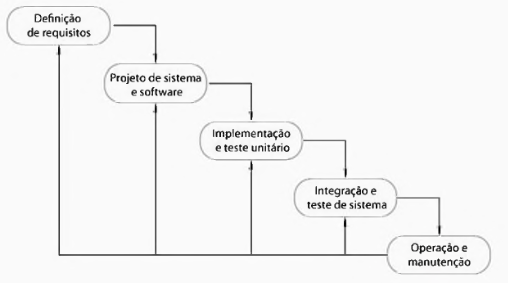
\includegraphics[width=8cm]{assets/modelo_cascata.png}
\end{figure}
%----------------------------------------------------------------------------

%----------------------------------------------------------------------------
\begin{figure}[h]
  \caption{Diagrama UML com os requisitos principais}

  \centering % para centralizarmos a figura
  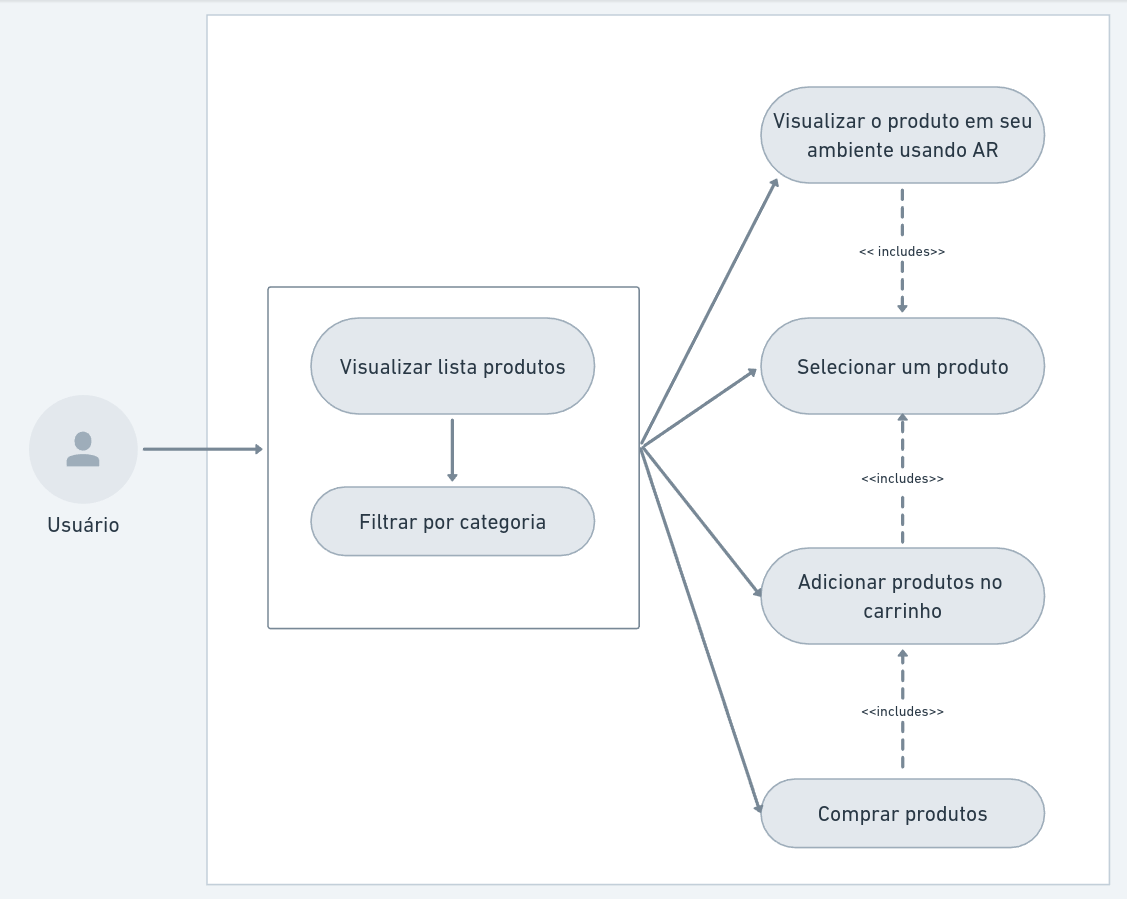
\includegraphics[width=8cm]{assets/user_uml_diagram.png}
\end{figure}
%----------------------------------------------------------------------------

\begin{thebibliography}{00}
  \bibitem{b}L. Tremosa. “Beyond AR vs. VR: What is the Difference between AR vs. MR vs. VR vs. XR?” Interaction Design Foundation - IxDF. https://www.interaction-design.org/literature/article/beyond-ar-vs-vr-what-is-the-difference-between-ar-vs-mr-vs-vr-vs-xr (accessed May. 30, 2024).

  \bibitem{b}J. Y. Ma and J. S. Choi, "The Virtuality and Reality of Augmented Reality," Journal of Multimedia, vol. 2, no. 1, pp. 32-37, 2007.

  \bibitem{sommerville2011engenharia}I. Sommerville, \emph{Engenharia de Software}. Pearson Prentice Hall, 2011. Available: https://books.google.com.br/books?id=H4u5ygAACAAJ

\end{thebibliography}

\end{document}
